% Ergänzung des Eraser-Diagramms um einen vierten Modelladapter.
% Die unveränderte Eraser-Grafik bleibt als Hintergrund erhalten.
% Positionen und Farben entsprechen der zugehörigen .eraser.json-Datei.
\documentclass[tikz,border=0pt]{standalone}
\usepackage[utf8]{inputenc}
\usepackage[T1]{fontenc}
\usepackage{graphicx}
\usepackage{helvet}
\renewcommand{\familydefault}{\sfdefault}
\definecolor{modellrahmen}{HTML}{ECC9A3}
\definecolor{modellflaeche}{HTML}{FDF0E1}
\definecolor{modelltext}{HTML}{374151}
\definecolor{nebentext}{HTML}{6B7280}
\begin{document}
\begin{tikzpicture}[x=1bp,y=1bp]
    \node[anchor=south west,inner sep=0pt,outer sep=0pt] at (0,0)
        {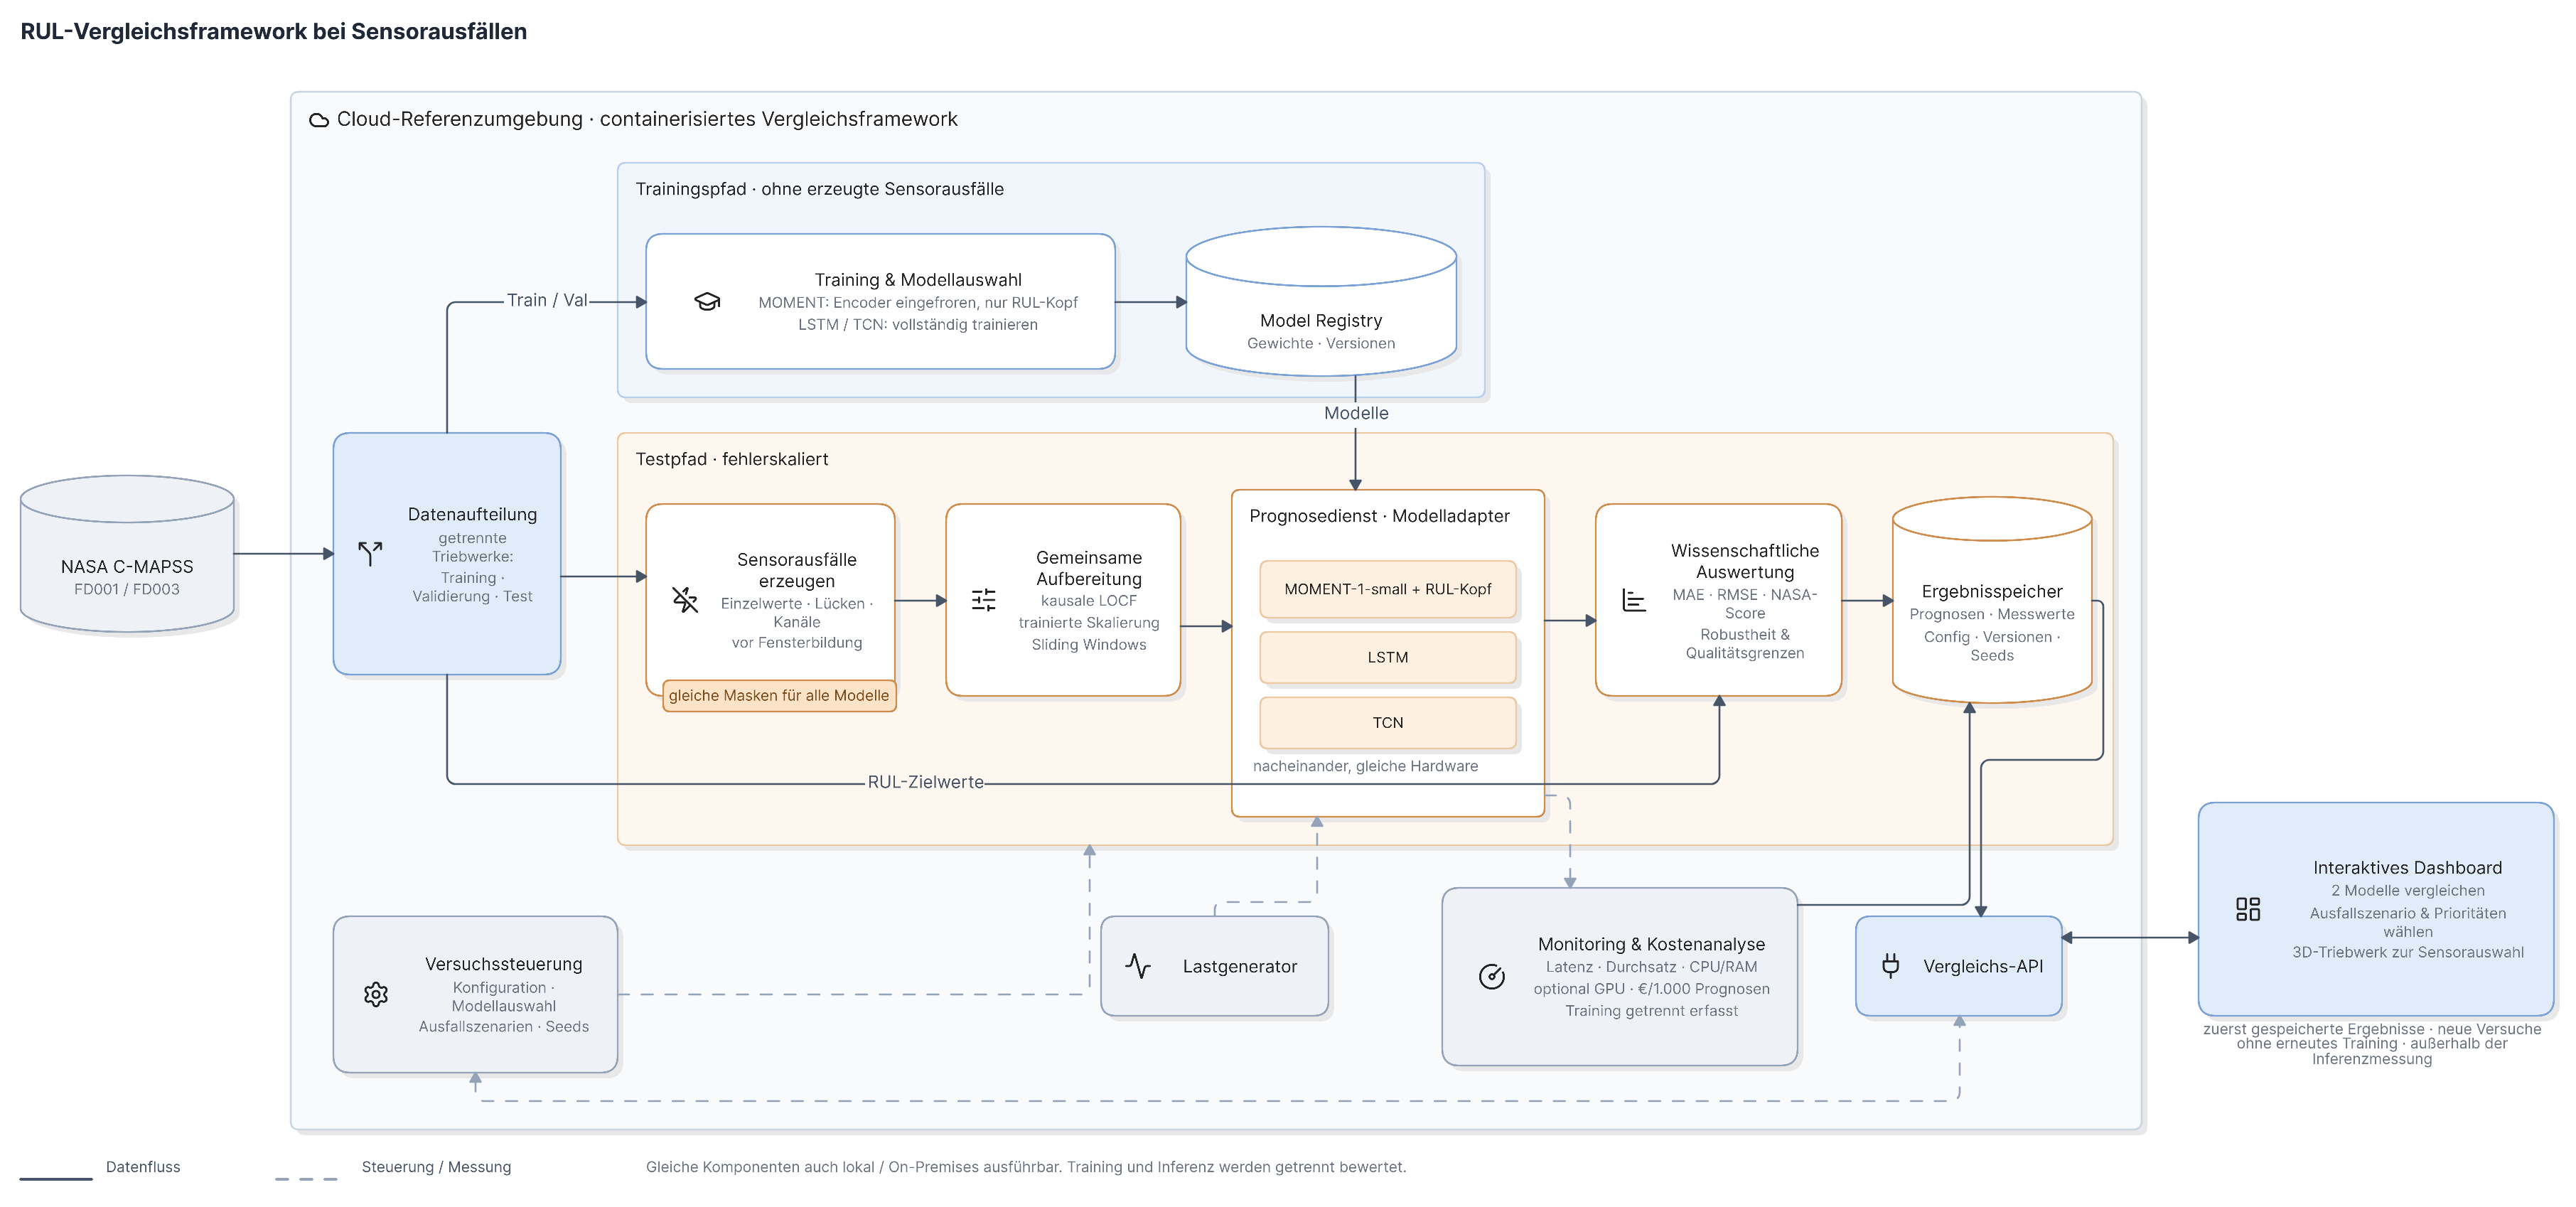
\includegraphics[width=1812bp,height=849bp]{architektur_rul_vergleichsframework.png}};
    \begin{scope}[yshift=849bp,yscale=-1]
        % Zusätzlicher vollständig trainierter Ansatz im Trainingspfad.
        \fill[white] (525,219) rectangle (777,235);
        \node[text=nebentext,font=\fontsize{12bp}{14bp}\selectfont,inner sep=0pt]
            at (646,228.5) {LSTM / TCN / Mamba: vollständig trainieren};
        % Vier Adapter innerhalb des bestehenden Prognosedienstes.
        \fill[white] (884,392) rectangle (1073,533);
        \fill[black,opacity=0.08,rounded corners=4bp] (890,398) rectangle (1070,426);
        \draw[draw=modellrahmen,fill=modellflaeche,line width=1bp,rounded corners=4bp] (887,395) rectangle (1067,423);
        \node[text=modelltext,font=\fontsize{12bp}{14bp}\selectfont,inner sep=0pt] at (977,409) {MOMENT-1-small + RUL-Kopf};
        \fill[black,opacity=0.08,rounded corners=4bp] (890,433) rectangle (1070,461);
        \draw[draw=modellrahmen,fill=modellflaeche,line width=1bp,rounded corners=4bp] (887,430) rectangle (1067,458);
        \node[text=modelltext,font=\fontsize{12bp}{14bp}\selectfont,inner sep=0pt] at (977,444) {LSTM};
        \fill[black,opacity=0.08,rounded corners=4bp] (890,468) rectangle (1070,496);
        \draw[draw=modellrahmen,fill=modellflaeche,line width=1bp,rounded corners=4bp] (887,465) rectangle (1067,493);
        \node[text=modelltext,font=\fontsize{12bp}{14bp}\selectfont,inner sep=0pt] at (977,479) {TCN};
        \fill[black,opacity=0.08,rounded corners=4bp] (890,503) rectangle (1070,531);
        \draw[draw=modellrahmen,fill=modellflaeche,line width=1bp,rounded corners=4bp] (887,500) rectangle (1067,528);
        \node[text=modelltext,font=\fontsize{12bp}{14bp}\selectfont,inner sep=0pt] at (977,514) {Mamba};
    \end{scope}
\end{tikzpicture}
\end{document}
